%
\documentclass[12pt]{amsart}
%\usepackage{txfonts}      %{article} was 12pt latex e
\usepackage{amssymb}
\usepackage{eucal}
\usepackage{amsmath}
\usepackage{amscd}
\usepackage[dvips]{color}
\usepackage{multicol}
\usepackage[all]{xy}           %xypic macro for latex2.09
\usepackage{graphicx}
\usepackage{color}
\usepackage{colordvi}
\usepackage{xspace}
\usepackage{listings}
\usepackage{framed}
\usepackage{lipsum}
%\usepackage{axodraw}
\usepackage{hyperref}
\hypersetup{colorlinks=true, urlcolor=cyan}

\usepackage[active]{srcltx} %SRC Specials for DVI Searching


\renewcommand\baselinestretch{1}    %was    1, 1.5 for double sp

%%standard setting
%\topmargin -0.3truein \textheight 8.4truein \oddsidemargin 0.2truein
%\evensidemargin 0.2truein \textwidth 440pt
%=========================================================================================
%%little larger standard setting: good setting
\topmargin -.8cm \textheight 22.8cm \oddsidemargin 0cm
\evensidemargin -0cm \textwidth 16.3cm
%==================================================================================
%% facing large setting
%\topmargin -.8cm \textheight 22.8cm \oddsidemargin -2cm
%\evensidemargin 2cm \textwidth 15cm
%==================================================================================
%%wide %% small font, fit window
%\topmargin -3.3cm \textheight 27.5cm \oddsidemargin -2cm
%\evensidemargin -2cm \textwidth 20cm
%%%%%%%%%%%%%%%================================================
%note setting, fit window
%%wide note setting, fit window
%\topmargin -1.6cm \textheight 23cm \oddsidemargin -0.9cm
%\textwidth 33cm \evensidemargin -0.9cm
%==================================================================================
%%wide note setting, no margin
%\topmargin -1.6cm \textheight 14.25cm \oddsidemargin -2cm
%\textwidth 20cm \evensidemargin -1.9cm
%=================================================================================%
%print narrow note setting
%\topmargin -0.5truein \textheight 9.8truein \oddsidemargin -0.7truein \evensidemargin -0.7truein \textwidth 340pt
%=================================================================================
%\makeatletter

%\makeatletter

\begin{document}  %for latex 2.09
%\input amssym.def %
%\input amssym      %

\newcommand{\nc}{\newcommand}
\newcommand{\delete}[1]{}
\nc{\dfootnote}[1]{{}}          %{{}}
\nc{\ffootnote}[1]{\dfootnote{#1}}
%\nc{\mfootnote}[1]{{}}        % Use this to suppress footnotes
\nc{\mfootnote}[1]{\footnote{#1}} % Use this to show footnotes
\nc{\todo}[1]{\tred{To do:} #1}

%\delete{
\nc{\mlabel}[1]{\label{#1}}  % Use this to suppress names
\nc{\mcite}[1]{\cite{#1}}  % Use this to suppress names
\nc{\mref}[1]{\ref{#1}}  % Use this to suppress names
\nc{\mbibitem}[1]{\bibitem{#1}} % Use this to show number
%}


\delete{
\nc{\mlabel}[1]{\label{#1}  % Use the next two lines to show names
{\hfill \hspace{1cm}{\bf{{\ }\hfill(#1)}}}}
\nc{\mcite}[1]{\cite{#1}{{\bf{{\ }(#1)}}}}  % Use this lines to show names
\nc{\mref}[1]{\ref{#1}{{\bf{{\ }(#1)}}}}  % Use this lines to show names
\nc{\mbibitem}[1]{\bibitem[\bf #1]{#1}} % Use this to show name
}

\nc{\mkeep}[1]{\marginpar{{\bf #1}}} % Use this to show marginpar
%\nc{\mkeep}[1]{{}}      % Use this to suppress marginpar

%%%%%%%%%%%%%%%%%%%%%%%% Statements
\newtheorem{theorem}{Theorem}[section]
%\newtheorem{prop}{Proposition}[section]
\newtheorem{prop}[theorem]{Proposition}
%\newtheorem{defn}{Definition}[section]
\newtheorem{defn}[theorem]{Definition}
\newtheorem{lemma}[theorem]{Lemma}
\newtheorem{coro}[theorem]{Corollary}
\newtheorem{prop-def}[theorem]{Proposition-Definition}
\newtheorem{claim}{Claim}[section]
\newtheorem{remark}[theorem]{Remark}
\newtheorem{propprop}{Proposed Proposition}[section]
\newtheorem{conjecture}{Conjecture}
\newtheorem{exam}[theorem]{Example}
\newtheorem{assumption}{Assumption}
\newtheorem{condition}[theorem]{Assumption}

\renewcommand{\labelenumi}{{\rm(\roman{enumi})}}
\renewcommand{\theenumi}{\roman{enumi}}

\newcommand{\vectornorm}[1]{\left|\left|#1\right|\right|}

\nc{\tred}[1]{\textcolor{red}{#1}}
\nc{\tblue}[1]{\textcolor{blue}{#1}}
\nc{\tgreen}[1]{\textcolor{green}{#1}}
\nc{\tpurple}[1]{\textcolor{purple}{#1}}
\nc{\btred}[1]{\textcolor{red}{\bf #1}}
\nc{\btblue}[1]{\textcolor{blue}{\bf #1}}
\nc{\btgreen}[1]{\textcolor{green}{\bf #1}}
\nc{\btpurple}[1]{\textcolor{purple}{\bf #1}}

\nc{\li}[1]{\textcolor{red}{Li:#1}}
\nc{\cm}[1]{\textcolor{blue}{Chengming: #1}}
\nc{\xiang}[1]{\textcolor{green}{Xiang: #1}}


%%%%%%%%%%%%%%%%%%%%%%% symbols
\nc{\adec}{\check{;}} \nc{\aop}{\alpha}
\nc{\dftimes}{\widetilde{\otimes}} \nc{\dfl}{\succ}
\nc{\dfr}{\prec} \nc{\dfc}{\circ} \nc{\dfb}{\bullet}
\nc{\dft}{\star} \nc{\dfcf}{{\mathbf k}} \nc{\spr}{\cdot}
\nc{\twopr}{\circ} \nc{\tspr}{\star} \nc{\sempr}{\ast}
\nc{\disp}[1]{\displaystyle{#1}}
\nc{\bin}[2]{ (_{\stackrel{\scs{#1}}{\scs{#2}}})}  %binomial coeff
\nc{\binc}[2]{ \left (\!\! \begin{array}{c} \scs{#1}\\
    \scs{#2} \end{array}\!\! \right )}  %binomial coeff
\nc{\bincc}[2]{  \left ( {\scs{#1} \atop
    \vspace{-.5cm}\scs{#2}} \right )}  %binomial coeff
\nc{\sarray}[2]{\begin{array}{c}#1 \vspace{.1cm}\\ \hline
    \vspace{-.35cm} \\ #2 \end{array}}
\nc{\bs}{\bar{S}} \nc{\dcup}{\stackrel{\bullet}{\cup}}
\nc{\dbigcup}{\stackrel{\bullet}{\bigcup}} \nc{\etree}{\big |}
\nc{\la}{\longrightarrow} \nc{\fe}{\'{e}} \nc{\rar}{\rightarrow}
\nc{\dar}{\downarrow} \nc{\dap}[1]{\downarrow
\rlap{$\scriptstyle{#1}$}} \nc{\uap}[1]{\uparrow
\rlap{$\scriptstyle{#1}$}} \nc{\defeq}{\stackrel{\rm def}{=}}
\nc{\dis}[1]{\displaystyle{#1}} \nc{\dotcup}{\,
\displaystyle{\bigcup^\bullet}\ } \nc{\sdotcup}{\tiny{
\displaystyle{\bigcup^\bullet}\ }} \nc{\hcm}{\ \hat{,}\ }
\nc{\hcirc}{\hat{\circ}} \nc{\hts}{\hat{\shpr}}
\nc{\lts}{\stackrel{\leftarrow}{\shpr}}
\nc{\rts}{\stackrel{\rightarrow}{\shpr}} \nc{\lleft}{[}
\nc{\lright}{]} \nc{\uni}[1]{\tilde{#1}} \nc{\wor}[1]{\check{#1}}
\nc{\free}[1]{\bar{#1}} \nc{\den}[1]{\check{#1}} \nc{\lrpa}{\wr}
\nc{\curlyl}{\left \{ \begin{array}{c} {} \\ {} \end{array}
    \right .  \!\!\!\!\!\!\!}
\nc{\curlyr}{ \!\!\!\!\!\!\!
    \left . \begin{array}{c} {} \\ {} \end{array}
    \right \} }
\nc{\leaf}{\ell}       % number of leafs
\nc{\longmid}{\left | \begin{array}{c} {} \\ {} \end{array}
    \right . \!\!\!\!\!\!\!}
\nc{\ot}{\otimes} \nc{\sot}{{\scriptstyle{\ot}}}
\nc{\otm}{\overline{\ot}} \nc{\ora}[1]{\stackrel{#1}{\rar}}
\nc{\ola}[1]{\stackrel{#1}{\la}}%${\Bbb Z}$
\nc{\pltree}{\calt^\pl} \nc{\epltree}{\calt^{\pl,\NC}}
\nc{\rbpltree}{\calt^r} \nc{\scs}[1]{\scriptstyle{#1}}
\nc{\mrm}[1]{{\rm #1}}
\nc{\dirlim}{\displaystyle{\lim_{\longrightarrow}}\,}
\nc{\invlim}{\displaystyle{\lim_{\longleftarrow}}\,}
\nc{\mvp}{\vspace{0.5cm}} \nc{\svp}{\vspace{2cm}}
\nc{\vp}{\vspace{8cm}} \nc{\proofbegin}{\noindent{\bf Proof: }}
%\nc{\proofbegin}{\begin{proof}} % AMS command
\nc{\proofend}{$\blacksquare$ \vspace{0.5cm}}
%\nc{\proofend}{\end{proof}} %AMS command
\nc{\freerbpl}{{F^{\mathrm RBPL}}}
\nc{\sha}{{\mbox{\cyr X}}}  %used to be \cyr
\nc{\ncsha}{{\mbox{\cyr X}^{\mathrm NC}}} \nc{\ncshao}{{\mbox{\cyr
X}^{\mathrm NC,\,0}}} \nc{\rpr}{\circ} \nc{\apr}{\cdot}
\nc{\dpr}{{\tiny\diamond}} \nc{\rprpm}{{\rpr}}
\nc{\shpr}{\diamond}    %Shuffle product
\nc{\shprm}{\overline{\diamond}}    %Shuffle product
\nc{\shpro}{\diamond^0}    %Shuffle product
\nc{\shprr}{\diamond^r}     %product on controlled trees
\nc{\shpra}{\overline{\diamond}^r} \nc{\shpru}{\check{\diamond}}
\nc{\catpr}{\diamond_l} \nc{\rcatpr}{\diamond_r}
\nc{\lapr}{\diamond_a} \nc{\sqcupm}{\ot} \nc{\lepr}{\diamond_e}
\nc{\vep}{\varepsilon} \nc{\labs}{\mid\!} \nc{\rabs}{\!\mid}
\nc{\hsha}{\widehat{\sha}} \nc{\lsha}{\stackrel{\leftarrow}{\sha}}
\nc{\rsha}{\stackrel{\rightarrow}{\sha}} \nc{\lc}{\lfloor}
\nc{\rc}{\rfloor} \nc{\tpr}{\sqcup} \nc{\nctpr}{\vee}
\nc{\plpr}{\star} \nc{\rbplpr}{\bar{\plpr}} \nc{\sqmon}[1]{\langle
#1\rangle} \nc{\forest}{\calf} \nc{\ass}[1]{\alpha({#1})}
\nc{\altx}{\Lambda_X} \nc{\vecT}{\vec{T}} \nc{\onetree}{\bullet}
\nc{\Ao}{\check{A}} \nc{\seta}{\underline{\Ao}}
\nc{\deltaa}{\overline{\delta}} \nc{\trho}{\tilde{\rho}}


%%%%%%%%%%%%%%%%%%%%% roman fonts, in alphabetic order
\nc{\mmbox}[1]{\mbox{\ #1\ }} \nc{\ann}{\mrm{ann}}
\nc{\Aut}{\mrm{Aut}} \nc{\can}{\mrm{can}} \nc{\twoalg}{{two-sided
algebra}\xspace} \nc{\bwt}{{mass}\xspace}
\nc{\bop}{{modification}\xspace} \nc{\ewt}{{mass}\xspace}
\nc{\ewts}{{masses}\xspace} \nc{\tto}{{extended}\xspace}
\nc{\Tto}{{Extended}\xspace} \nc{\tte}{{extended}\xspace}
\nc{\gyb}{{generalized}\xspace} \nc{\Gyb}{{Generalized}\xspace}
\nc{\MAYBE}{{EAYBE}\xspace} \nc{\GAYBE}{{GAYBE}\xspace}
\nc{\esym}{\vep} \nc{\colim}{\mrm{colim}} \nc{\Cont}{\mrm{Cont}}
\nc{\rchar}{\mrm{char}} \nc{\cok}{\mrm{coker}} \nc{\dtf}{{R-{\rm
tf}}} \nc{\dtor}{{R-{\rm tor}}}
\renewcommand{\det}{\mrm{det}}
\nc{\depth}{{\mrm d}} \nc{\Div}{{\mrm Div}} \nc{\End}{\mrm{End}}
\nc{\Ext}{\mrm{Ext}} \nc{\Fil}{\mrm{Fil}} \nc{\Frob}{\mrm{Frob}}
\nc{\Gal}{\mrm{Gal}} \nc{\GL}{\mrm{GL}} \nc{\Hom}{\mrm{Hom}}
\nc{\hsr}{\mrm{H}} \nc{\hpol}{\mrm{HP}} \nc{\id}{\mrm{id}}
\nc{\im}{\mrm{im}} \nc{\incl}{\mrm{incl}}
\nc{\length}{\mrm{length}} \nc{\LR}{\mrm{LR}} \nc{\mchar}{\rm
char} \nc{\NC}{\mrm{NC}} \nc{\mpart}{\mrm{part}}
\nc{\pl}{\mrm{PL}} \nc{\ql}{{\QQ_\ell}} \nc{\qp}{{\QQ_p}}
\nc{\rank}{\mrm{rank}} \nc{\rba}{\rm{RBA }} \nc{\rbas}{\rm{RBAs }}
\nc{\rbpl}{\mrm{RBPL}} \nc{\rbw}{\rm{RBW }} \nc{\rbws}{\rm{RBWs }}
\nc{\rcot}{\mrm{cot}} \nc{\rest}{\rm{controlled}\xspace}
\nc{\rdef}{\mrm{def}} \nc{\rdiv}{{\rm div}} \nc{\rtf}{{\rm tf}}
\nc{\rtor}{{\rm tor}} \nc{\res}{\mrm{res}} \nc{\SL}{\mrm{SL}}
\nc{\Spec}{\mrm{Spec}} \nc{\tor}{\mrm{tor}} \nc{\Tr}{\mrm{Tr}}
\nc{\mtr}{\mrm{sk}} \nc{\type}{{\bwt}\xspace}

%%%%%%%%%%%%%%%%%% bold face
\nc{\ab}{\mathbf{Ab}} \nc{\Alg}{\mathbf{Alg}}
\nc{\Algo}{\mathbf{Alg}^0} \nc{\Bax}{\mathbf{Bax}}
\nc{\Baxo}{\mathbf{Bax}^0} \nc{\RB}{\mathbf{RB}}
\nc{\RBo}{\mathbf{RB}^0} \nc{\BRB}{\mathbf{RB}}
\nc{\Dend}{\mathbf{DD}} \nc{\bfk}{{\bf k}} \nc{\bfone}{{\bf 1}}
\nc{\base}[1]{{a_{#1}}} \nc{\detail}{\marginpar{\bf More detail}
    \noindent{\bf Need more detail!}
    \svp}
\nc{\Diff}{\mathbf{Diff}} \nc{\gap}{\marginpar{\bf
Incomplete}\noindent{\bf Incomplete!!}
    \svp}
\nc{\FMod}{\mathbf{FMod}} \nc{\mset}{\mathbf{MSet}}
\nc{\rb}{\mathrm{RB}} \nc{\Int}{\mathbf{Int}}
\nc{\Mon}{\mathbf{Mon}}
%\nc{\remark}{\noindent{\bf Remark: }}
\nc{\remarks}{\noindent{\bf Remarks: }}
\nc{\OS}{\mathbf{OS}} %free operated semigroup
\nc{\Rep}{\mathbf{Rep}} \nc{\Rings}{\mathbf{Rings}}
\nc{\Sets}{\mathbf{Sets}} \nc{\DT}{\mathbf{DT}}

%%%%%%%%%%%%%%%%%%%Bbb fonts
\nc{\BA}{{\mathbb A}} \nc{\CC}{{\mathbb C}} \nc{\DD}{{\mathbb D}}
\nc{\EE}{{\mathbb E}} \nc{\FF}{{\mathbb F}} \nc{\GG}{{\mathbb G}}
\nc{\HH}{{\mathbb H}} \nc{\LL}{{\mathbb L}} \nc{\NN}{{\mathbb N}}
\nc{\QQ}{{\mathbb Q}} \nc{\RR}{{\mathbb R}} \nc{\TT}{{\mathbb T}}
\nc{\VV}{{\mathbb V}} \nc{\ZZ}{{\mathbb Z}}


%%%%%%%%%%%%%%%%%%% cal fonts

\nc{\calao}{{\mathcal A}} \nc{\cala}{{\mathcal A}}
\nc{\calc}{{\mathcal C}} \nc{\cald}{{\mathcal D}}
\nc{\cale}{{\mathcal E}} \nc{\calf}{{\mathcal F}}
\nc{\calfr}{{{\mathcal F}^{\,r}}} \nc{\calfo}{{\mathcal F}^0}
\nc{\calfro}{{\mathcal F}^{\,r,0}} \nc{\oF}{\overline{F}}
\nc{\calg}{{\mathcal G}} \nc{\calh}{{\mathcal H}}
\nc{\cali}{{\mathcal I}} \nc{\calj}{{\mathcal J}}
\nc{\call}{{\mathcal L}} \nc{\calm}{{\mathcal M}}
\nc{\caln}{{\mathcal N}} \nc{\calo}{{\mathcal O}}
\nc{\calp}{{\mathcal P}} \nc{\calr}{{\mathcal R}}
\nc{\calt}{{\mathcal T}} \nc{\caltr}{{\mathcal T}^{\,r}}
\nc{\calu}{{\mathcal U}} \nc{\calv}{{\mathcal V}}
\nc{\calw}{{\mathcal W}} \nc{\calx}{{\mathcal X}}
\nc{\CA}{\mathcal{A}}


%%%%%%%%%%%%%%%%%%  frak fonts
\nc{\fraka}{{\mathfrak a}} \nc{\frakB}{{\mathfrak B}}
\nc{\frakb}{{\mathfrak b}} \nc{\frakd}{{\mathfrak d}}
\nc{\oD}{\overline{D}} \nc{\frakF}{{\mathfrak F}}
\nc{\frakg}{{\mathfrak g}} \nc{\frakk}{{\mathfrak k}}
\nc{\frakm}{{\mathfrak m}} \nc{\frakM}{{\mathfrak M}}
\nc{\frakMo}{{\mathfrak M}^0} \nc{\frakp}{{\mathfrak p}}
\nc{\frakS}{{\mathfrak S}} \nc{\frakSo}{{\mathfrak S}^0}
\nc{\fraks}{{\mathfrak s}} \nc{\os}{\overline{\fraks}}
\nc{\frakT}{{\mathfrak T}} \nc{\oT}{\overline{T}}
%\nc{\frakx}{{\mathfrak x}}
\nc{\frakX}{{\mathfrak X}} \nc{\frakXo}{{\mathfrak X}^0}
\nc{\frakx}{{\mathbf x}}
%\nc{\frakTxo}{{\frakTx}^0}
\nc{\frakTx}{\frakT}      %All rooted trees, correspond to \ncsha(X)
\nc{\frakTa}{\frakT^a}        % rooted trees for \ncsha(A)
\nc{\frakTxo}{\frakTx^0}   % rooted trees for \ncshao(X)
\nc{\caltao}{\calt^{a,0}}   % rooted trees for \ncshao(A)
\nc{\ox}{\overline{\frakx}} \nc{\fraky}{{\mathfrak y}}
\nc{\frakz}{{\mathfrak z}} \nc{\oX}{\overline{X}}

\font\cyr=wncyr10

\nc{\redtext}[1]{\textcolor{red}{#1}}


%%%%%%%%%%%%%%%%%%%%%%%%%%%%%%%%%%%%%%%%%%%%%%%%%%%%%%%%%%%%%%%%%%




\hfil {\bf \Huge{Qishi quiz 2}}\hfil





\bigskip

\hfil {Group 2} \hfil




\bigskip



\section{Problem 1}

$\chi^2$ test is any statistical hypothesis test in which the sampling distribution of the test statistic is a $\chi^2$ distribution when the null hypothesis is true. It can be used to test the residuals distribution of model fitting.

The $\chi^2$ test static is :
\begin{equation*}
	\chi^2 = \sum_{i=1}^n \frac{(O_i - E_i)^2}{E_i}
\end{equation*}

Where $n$ is the number of observation, $O_i$ is the observed frequency of outcome i. $E_i$ is the expected frequency of outcome i. Once we get $\chi^2$ we can calculate the corresponding p-value of $\chi^2$ distribution with dof $k=n-q-1$.

If p-value is smaller than certain conventional criteria say 0.05, we can reject the null hypothesis(normal distribution).




\section{Problem 2}
This is a Chinese postman problem. For a 2 by 3 grid we have 6 vertices with odd order which are 2,3,5,8,10,11. We can make it a semi Eulerian graph by connecting 2-3 and 10-11 directly. Now we can start from 5 and end at 8 to traverse all edges of the new graph. The length of the path will be 17+2=19.

\begin{framed}
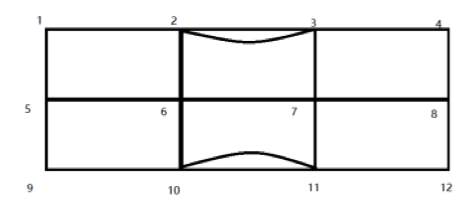
\includegraphics[width=10cm]{P2-tianmu.png}
\end{framed}




\section{Problem 3}
%Let $Z=X+Y$. Since $X,Y$ are iid $N(0,1)$, $Z$ is normal with mean $0$ and variance $2$. Moreover by symmetry we have $P(X|X+Y>0)=P(Y|X+Y>0)$. So $P(X|X+Y>0)=\frac{1}{2}P(X+Y|X+Y>0)=\frac{1}{2}P(Z|Z>0)=\frac{1}{2}\cdot(\frac{1}{2\sqrt{\pi}}\int_{0}^{\infty}xe^{-\frac{x^2}{4}}dx)/P(Z>0)=\frac{1}{2\sqrt{\pi}}\int_{0}^{\infty}xe^{-\frac{x^2}{4}}dx=\frac{1}{\sqrt{\pi}}\int_{0}^{\infty}e^{-\frac{x^2}{4}}d(\frac{x^2}{4})=-\frac{1}{\sqrt{\pi}}e^{-y}|_0^{\infty}=\frac{1}{\sqrt{\pi}}$. So $P(X|X+Y>0)=\frac{1}{\sqrt{\pi}}$.

X and Y are iid N(0,1).
\begin{eqnarray*}
	P(X|X+Y>0) &=& P(X \cap X+Y>0)/P(X+Y>0) \\
	&=& P(X)P(Y>-X) \\
	&=& \frac{ \frac{1}{\sqrt{2\pi}}e^{-\frac{x^2}{2}} \int_{-x}^\infty \frac{1}{\sqrt{2\pi}}e^{-\frac{y^2}{2}dy}}{0.5} \\
	&=& \sqrt{\frac{2}{\pi}} e^{-\frac{x^2}{2}} (1- \Phi(-x)) \\
	&=& \sqrt{\frac{2}{\pi}} e^{-\frac{x^2}{2}} \Phi(x)
\end{eqnarray*}

\section{Problem 4}
(1) If keep rolling for once, the payoff is $0$ with probability $1/6$ and is $35+i$ for $i=2,...6$ with probability $1/6$ respectively. In this case the expected payoff is $\frac{1}{6}\cdot\sum_{i=2}^6(35+i)=32.5$. Since by rolling once, the maxmimum sum we can get is $35+6=41$ and $41+6=47<7^2=49$, we could still keep rolling without worrying about to get a square. After rolling twice the payoff become $32.5+3.5=36$ which is geater than $35$. Hence we should keep rolling if the sum is 35. 

(2) If we get $2$, then we could continue rolling at least twice and in this case the most possible number to get is 7+2=9. Fo the other cases $3,4,5,6$ we get the same results. Since the probability to get $2,3,4,5,6$ are the same, the most possible number is $35+9=44$.

(3) Suppose we arrive at $n^2-6\leq k\leq n^2$, then if we stop we at least get $n^2-6$. If we continue we could nearly get $(n+1)^2-1$ with probability at most $5/6$. So we stop when we have $n^2-6>5/6(n^2-2n)$ which implies $n\geq 13$. So we stop between $163$ and 169. 

\section{Problem 5}
The two breaking points $x$ and $y$ are uniformlly distributed on $[0,1]$. Let $c_1,c_2,c_3$ be the length of each piece. Then $c_1+c_2+c_2<1$ and the area of volumn of it is $1/3!=1/6$. So the joint distribution of them is $1/6$. Let $A=min(X,Y), B=max(X,Y)$ and $C=min(A,1-B,B-A)$. Let $F_C(a)$ be the cdf of $C$. Then $1-F_C(a)=Prob(C\geq a) = P(a\leq X\leq 1,a\leq Y\leq 1-a,|X-Y|\geq a)=1-(1-3a)^2$. So the pdf of $C$ is $f_C(a)=F_C'(a)=6(1-3a)$. So the expected length of the smallest piece is $\int_0^{1/3}6a(1-3a)da=1/9$.

Similarly we can compute the expected length of the longest piece. Let $D=max(A,1-B,B-a)$. Then the cdf for $D$ is $F_D(a)=Prob(D\leq a)=Prob(A\leq a,1-B\leq a,B-A\leq a)$. So $F_D(a)=(3a-1)^2$ if $1/3\leq a\leq 1/2$ and $F_D(a)=1-3(1-a)^2$ if $1/2\leq a\leq 1$. So the pdf of $D$ is $f_D(a)=6(3a-1)$ if $1/3\leq a\leq 1/2$ and $f_D(a)=6(1-a)$ if $1/2\leq a\leq 1$. So the expected length of the longest piece is 
$\int_{1/3}^{1/2}6a(3a-1)da + \int_{1/2}^16a(1-a)da = 11/18$. 

Hence, the expected length of the middle-sized piece is $1-1/9-11/18=5/18$.

\section{Problem 6}
(1) For $i=1,...,N$, define random variable $I_i=1$ if person $i$ choose his/her own hat and $I_i=0$ otherwise. Then $E(I_i)=Prob(I_i=1)=1/N$. Then $Y=\sum_iI_i$. So $E(Y)=E(\sum_iI_i)=\sum_i E(I_i)=N\cdot 1/N=1$.

(2) We have $E(Y^2)=E((\sum_iI_i)\cdot (\sum_jI_j) =E(\sum_{i,j=1}I_iI_j)=sum_{i,j=1}E(I_iI_j)=\sum_{i,j=1,i\neq j}Prob(I_i=1,I_j=1)+\sum_iProb(I_i=1)=\sum_{i,j=1,i\neq j}\frac{1}{N(N-1)}+\sum_iProb(I_i=1)\frac{1}{N}=1+1=2$. So the variance of Y is $var(Y)=E(Y^2)-(E(Y))^2=2-1^2=1$.

(3) Let $X_N$ be the random variable counting the nuber of people picking their own hats in the first round. Since from (1) we know that on average there are one person who picks his/her own hat, we might guess that be the number of rounds that are run are $R(N)=N$. In fact, it is easy to see that it is true for $N=1$. For general $N$, we could prove it by induction. In fact, suppose that it holds up to $N-1$. Then
\begin{eqnarray*}
E(R(N))&=&\sum_{i=0}^NE(R(N)|X_N=i)Prob(X_N=i)\\
&=&\sum_{i=0}^N(1+E(R(N-i))Prob(X_N=i)\\
&=&\sum_{i=0}^NProb(X_N=i)+E(R(N))Prob(X_N=0)+\sum_{i=1}^N(N-i)Prob(X_N=i)\\
&=&1+E(R(N))Prob(X_N=0)+N(1-Prob(X_N=0))-E(X_N)\\
&=&E(R(N)))Prob(X_N=0)+N(1-Prob(X_N=0)),
\end{eqnarray*}
where the third equality follows from induction hypothesis and the last equality follows from (1) that $E(X_N)=1$. So $E(R(N))(1-Prob(X_N=0))=N(1-Prob(X_N=0))$ which implies $E(R(N))=N$ since $P(X_N=0)\neq1$. This finishes the induction process.

(4)  Conditioning on $X_N$ gives
\begin{eqnarray*}
E(S(N))&=&\sum_{i=0}^NE(S(N)|X_N=i)Prob(X_N=i)\\
&=&\sum_{i=0}^N(N+E(S(N-i))Prob(X_N=i)\\
&=&N+\sum_{i=0}^NE(S(N-i)Prob(X_N=i).
\end{eqnarray*}
This implies $$E(S(N))=N+E(S(N-X_N)).$$ Because of this relation, it is natural to assume that $E(S(N))$ is a polynomial function of $N$. But if there is exactly only one match in each round, we would have $\sum_{i=1}^Ni=N(N+1)/2$  selections. So it would be natural to assume $E(S(N))$ is a quadratic polynomial function of $N$. So suppose that $E(S(N))= aN^2+bN$ and plug this into the above equation. We get 
$aN^2+bN=N+E(a(N-X_N)^2+b(N-X_N)]$. Since $E(X_N)=var(X_N)=1$, we have $aN^2+bN=aN^2+(b-2a+1)N+2a-b$. So $a=1/2$ and $b=1$. This implies $E(S(N))=N+N^2/2$. To prove it rigoriously, we could use induction. In the case of $N=2$, it is true because the number of rounds is geometric distribution with parameter $1/2$. Suppose that it is true up to $N-1$. Then
\begin{eqnarray*}
E(S(N))&=&N+E(S(N))Prob(X_N=0)+\sum_{i=1}^NE(S(N-i)Prob(X_N=i)\\
&=&N+E(S(N))Prob(X_N=0)+\sum_{i=1}^N((N-i)^2/2+(N-i))Prob(X_N=i)\\
&=&N+E(S(N))Prob(X_N=0)+(N^2/2+N)(1-Prob(X_N=0))-(N+1)E(X_N)\\
& &+E(X_N^2)/2
\end{eqnarray*}
where the second equality follows from induction hypoethesis. Plugging $E(X_N)=1,E(X_N^2)=2$ into the above equation gives $E(S(N))=N+N^2/2$, as desired.

(5)  Let $H_i$ be the randon variable counting the number of hats chosen by person $i$. Then $\sum_i H_i = S(N)$. Hence $E(\sum_iH_i)=E(S(N))$. By symmetry, $H_i$ has the same mean, so $E(H_i)=S(N)/N=1+n/2$. So the expected number of false selections made by
one of the N people is $E(H_i-1)=n/2$. 

\section{Problem 7}
The upper bound is 1 and the lower bound is 0.02.  Let $\iota$ be a column vector every element of which is 1. Let $x$ be a $n\times k$ matrix and let $S(x)$ be the subspace generated by the column vectors of $x$. Then
$P_x=x(x^Tx)^{-1}x^T$ is the projection matrix projecting onto $S(x)$ and $M_x=I-P_x=I-x(x^Tx)^{-1}x^T$ is the annihilator space projecting onto the orthogonal complement subspace $S^{\bot}(X)$. Then the (centered) $R^2$ is
$$R^2=\frac{\|P_xM_{\iota}y\|^2}{\|M_{\iota}y\|^2},$$
where $M_{\iota}y=(I-P_{\iota})y=y-\iota(\iota^T\iota)^{-1}\iota^Ty=y-\bar{y}\iota$ is the centered version of $y$ and $\bar{y}=\frac{1}{n}\sum_{t=1}^ny_t$ is the mean of $y$. Here we assume that $\iota$ is contained in the span $S(x)$ of the regressors. So in this problem
$S(x)$ is $S(x_1,\iota)$ or $S(x_2,\iota)$ or $S(x_1,x_2,\iota)$. 
 
 
 Upper bound: If $M_{\iota}y\in S(x_1,x_2)$, the vector space generated by the column vectors of $x_1$ and $x_2$, then $\|P_{(x_1,x_2)}M_{\iota}y\|^2=\|M_{\iota}y\|^2\Rightarrow R^2=1$. Since $R^2\leq 1$, the upper bound of $R^2$ is 1. Geometrically, this means that $M_{\iota}y$ belongs to the subspace span by (the column vectors of) $x_1$ and $x_2$, so the model is perfectly fit and $R^2=1$.
 
Lower bound: First we show that $R_{M_3}^2\geq R_{M_1}^2,R_{M_2}^2$, where we use subscripts to differentiate $R^2$ from different models. Without loss of generality, we just need to prove the case for $M_2$. In fact, since both $P_{x_1,x_2,\iota}$ and $P_{x_2,\iota}$ are symmetric, so is $P_{x_1,x_2,\iota}-P_{x_2,\iota}$. Moreover, since $S(x_2,\iota)\subset S(x_1,x_2,\iota)$, we have $P_{x_1,x_2,\iota}P_{x_2,\iota}=P_{x_2,\iota}P_{x_1,x_2,\iota}=P_{x_2,\iota}$. So $(P_{x_1,x_2,\iota}-P_{x_2,\iota})^2=
 P_{x_1,\iota,x_2,\iota}^2-P_{x_1,\iota,x_2,\iota}P_{x_2,\iota}
 -P_{x_2,\iota}P_{x_1,x_2,\iota}+P_{x_2,\iota}^2=P_{x_1,x_2,\iota}-P_{x_2,\iota}$
 as both of $P_{x_1,x_2,\iota}$ and $P_{x_2,\iota}$ are idempotents. So $P_{x_1,x_2,\iota}-P_{x_2,\iota}$ is an orthogonal projection matrix. 
  Hence   $\|P_{x_1,x_2,\iota}M_{\iota}y\|^2-
  \|P_{x_2,\iota}M_{\iota}y\|^2=(M_{\iota}y)^T(P_{x_1,x_2,\iota}
 -P_{x_2,\iota})M_{\iota}y=\|(P_{x_1,x_2,\iota}
 -P_{x_2,\iota})M_{\iota}y\|^2\geq0\Rightarrow \frac{\|P_{x_1,x_2,\iota}M_{\iota}y\|^2}{\|M_{\iota}y\|^2}\geq \frac{\|P_{x_2,\iota}M_{\iota}y\|^2}{\|M_{\iota}y\|^2}$. So $R_{M_3}^2\geq R_{M_2}^2=0.02$. But this equality can be attained. In fact, if 
$\|P_{x_1,x_2,\iota}M_{\iota}y\|^2=\|P_{x_2,\iota}M_{\iota}y\|^2$, then 
$R_{M_3}^2=0.02$. Geometrically, to do the OLS for model $M_3$, it amounts to find a
vector $v$ inside $S(x_1,x_2,\iota)$ such that $\|M_{\iota}y-v\|^2$ is minimized. In our case that $R_{M_3}^2=0.02$£¬ this minimization is exactly achieved by $P_{x_2,\iota}M_{\iota}y$.

So the range of $R^2$ of Model 3 is $[0.02, 1]$.


\section{Problem 8}
$1/n$ is a rational number so it can be written as binary number with finite sum: $1/n=\sum_{i=1}^mp_i2^{-i}$ for $p_i=0,1$. Then the function biasedCoin() can be implement (by using the function fairCoin()) in the following ways:


\begin{framed}
\lstinputlisting{quiz2Pro8.cpp}
\end{framed}
The algorithm is explained as follows: when we coss a fair coin, the heads count as 1 and the tails count as 0. Let $s_i\in\{0,1\}$ be the result of $i$-th toss starting with $i=1$. After each toss, we compare $s_i$ with $p_i$. If $s_i < p_i$ (resp. $s_i > p_i$), the baisedCoin() return a head (resp. tail) and the tossing stops. If $s_i=p_i$, we continue tossing the fair coin. If we end up with $s_n=p_n$, baisedCoin() return a tail. This will give a function which return heads with probabilty $1/n$.


\section{Problem 9}

There's a confusion that if the man gets on a weak bridge and fall, will it count as one cross? We won' count that in in our solution.

There are different understanding of this problem. If "miraculously fixed" means all bridges are fixed strong, then we have Xiang Ni's answer below:

Let $A_i$ be the event that the $i$-th bridge is weak and the previus $i-1$ bridges are all strong (i.e $i$ is the first weak bridge), then $A_i$ are disjoint and $P(\cup_{i=1}^{10}A_i)=1$, where $A_{10}$ means that all the bridges are strong. Moreover, we have $Prob(A_i)=\frac{1}{2^i}$ for $i\le 9 $ and $Prob(A_{10})=\frac{1}{2^{9}}$. Define random variables $I_i$ as $I_i=1$ on $A_i$ and $I_i=0$, otherwise. Let $X$ be the random variable counting how many brdges the man has to cross. Then $X|_{A_i}=i-1+9=i+8$ for $i\le 9$ and $X|_{A_{10}}=9$. So $E(X)=\sum_{i=1}^{9}(i+8)\cdot\frac{1}{2^i}+9\cdot\frac{1}{2^{9}} = 10-\frac{10}{2^9}$. So to arrive the 10th island, on average the man has to cross $10-\frac{10}{2^{9}}$ bridges.

If "miraculously fixed" means all bridges are "shuffled", including the broken bridge can now be strong or weak, we have Tianmu Xin's answer:

Use $E_i$ to denote the expected number of bridges one need to cross from ith island to 10th island. 
Then 
\begin{eqnarray*}
E_i = \frac{1}{2} (1+E_{i+1} )+\frac{1}{2} E_1	
\end{eqnarray*}
The first term means there is $1/2$ probability that one will make a cross from ith island to island i+1 by crossing one bridge and $1/2$ probability of starting over from 1st island. And we know that $E_10=0$. 
We can use $E_10$ to express $E_9$ and use $E_9$ to express $E_8$, so on so forth we can eventually express $E_1$ with $E_10$ as
\begin{eqnarray*}
E_1=\sum_{i=1}^8 \frac{1}{2^i} + \frac{1}{2^9}  (1+E_{10} )+\sum_{i=1}^9 \frac{1}{2^i}  E_1
\end{eqnarray*}
Solve this we can get
\begin{eqnarray*}
	E_1=2^9-1
\end{eqnarray*}


If "miraculously fixed" means only the broken bridge is fixed and is strong now, here is Cong Chen's answer:
The equation we have should be:
\begin{eqnarray*}
	E_i = \frac{1}{2}(1+E_{i+1}) + \frac{1}{2}(i + E_{i+1})
\end{eqnarray*}

And this gives us $E_1 = 27$.

\section{Problem 10}
const before * means the value the pointer points to is constant.

const after * means the address the pointer points to cannot be changed.

const at the end of class method declaration means this method cannot change any class members.

Reference:
\url{http://duramecho.com/ComputerInformation/WhyHowCppConst.html}

\section{Problem 11}
\begin{framed}
\lstinputlisting{quiz2Pro11.cpp}
\end{framed}



\section{Problem 12}
The .hh file for the matrix class is as follows:
\begin{framed}
\lstinputlisting{quiz2Pro12.hh}
\end{framed}
The .cpp file for the matrix class is as follows:
\begin{framed}
\lstinputlisting{quiz2Pro12.cpp}
\end{framed}


\section{Problem 13}

No,  constructor of a class CANNOT be virtual. Here is a quote from Bjarne Stroustrup's C++ Style and Technique FAQ: "{\em virtual call is a mechanism to get work done given partial information. In particular, "virtual" allows us to call a function knowing only any interfaces and not the exact type of the object. To create an object you need complete information. In particular, you need to know the exact type of what you want to create. Consequently, a "call to a constructor" cannot be virtual}."

When virtual function is called, compiler looks for the correct function in the vtable. Vtable is not constructed yet when constructor is firstly called so constructor cannot be virtual.

\begin{framed}
\lstinputlisting{P13.h}
\end{framed}

Reference of virtual constructor implementation:
\newline
\url{http://www.geeksforgeeks.org/advanced-c-virtual-constructor/}

\section{Problem 14}
Yes, but the non-virtual function was not redefined in any derived class.

Reference: \url{https://isocpp.org/wiki/faq/strange-inheritance#calling-virtuals-from-base}


\section{Problem 15}
Any single character is a palindrome. If the character after this character is the same, then they form a two char palindrome. If the characters before and after this palindrome are the same then we got a four char palindrome. 
We need a table to record whether the substring from i to j is a palindrome. 
$T[i,i]$ should be all true. Then check the consecutive char and see if T[i,i+1] is true. 
After that we need to go over every substring $T[i,j]$ and check if it is palindrome and if the chars before and after it are the same, if so we update the $T[i-1,j+1]$. Then we need to expand this to next possible length of the palindrome, Therefore this will have $O(N^2)$ time complexity. 

Cpp code provided by Tianmu Xin:
\begin{framed}
\lstinputlisting{P15.cpp}
\end{framed}


Python code provided by Xiang Ni:
\begin{framed}
\lstinputlisting{quiz2Pro15.py}
\end{framed}


\section{Problem 16}
We can first reverse the sentence and then reverse each words. The time complexity is $O(N^2)$.

\begin{framed}
\lstinputlisting{P16.py}
\end{framed}



\section{Problem 17}
Use dynamic programming. For each i, find the max profits profit1[i] and profits2[i] with one transection from prices[0] to prices[i] and from prices[i+1] to prices[n-1] respectively. Find the  maximal profit1[i]+profit2[i] from 0 to n-1. The time complexity is $O(N)$.

\begin{framed}
\lstinputlisting{P17.py}
\end{framed}


\section{Problem 18}
Form a graph such that each node represent each person and if two persons are friends, then there is an edge connecting the corresponding two nodes. Then this problem actually asks to find a Hamiltonian Path in this graph, that is a path that visits each vertex exactly once.
We could use back-tracking algorithm to find such path. The input is a $N$ by $N$ matrix graph[N][N] which is the adjacency matrix representation of the graph. A value graph[i][j] is 1 if there is a direct edge from i to j (i.e. person i and person j are friends), otherwise graph[i][j] is 0. 

\begin{framed}
\lstinputlisting{quiz2Prob18.py}
\end{framed}

%\begin{thebibliography}{abcdsfgh}





%\end{thebibliography}

\end{document}



